\documentclass[memoire.tex]{subfiles}
\begin{document}



\section*{Introduction}
Dans sa forme la plus générale, la théorie de la bifurcation (statique) pourrait se résumer aux différentes techniques mises en place pour répondre à la question suivante : Étant donné deux espaces abstraits $X$ et $Y$, un espace de paramètre $\Lambda$ et une famille de fonctions 
\begin{equation*}
    (f_{\lambda}: X\rightarrow Y)_{\lambda\in\Lambda}
\end{equation*} comment le lieu $f^{-1}_{\lambda}(0)$ change-t-il quand $\lambda$ varie ? On peut réécrire cette famille de fonctions comme une fonction 
$F: X\times\Lambda\rightarrow Y$. Il faut bien sûr préciser un peu ce que sont ces espaces, sans quoi, on ne peut rien dire.\\Nous supposerons que les outils de base du calcul différentiel s'appliquent confortablement à $X$ et $Y$ et nous verrons que pour ce faire, il faut supposer que ce sont des espaces de Banach.\\
Historiquement, ce type de problème apparut lors de l'étude de systèmes dynamiques dont la loi d'évolution dépend d'un paramètre. Précisons: 
considérons l'équation différentielle suivante :
\begin{equation}\label{equanewton}
    \frac{\partial  x}{\partial t }= F(x,\lambda)
\end{equation}
en supposant, par exemple, $x:\R\rightarrow \R^n$ et $\lambda\in\R$. On peut s'intéresser, dans un premier temps, aux \coldef{équilibres} de ce système, naturellement, cela correspond à étudier 
$F_{\lambda}^{-1}(0)$. Considérons le cas très simple d'un mobile ayant un seul degré de liberté, et 
\begin{equation*}
    F(x,\lambda)= x^3-\lambda x
\end{equation*}
On constate immédiatement 
que le nombre de points 
d'équilibres passe de 1 à 3 
quand $\lambda$ devient 
positif. Remarquons déjà 
qu'ici une partie du lieu 
d'annulation de $F$ est 
assez inintéressante. En 
effet, il est évident que 
si $x=0$ alors $F(x,\lambda)
=0$, dans la suite, cette 
branche de solution 
inintéressante sera 
qualifiée de branche 
triviale et la majorité du 
travail consistera à étudier 
les \coldef{bifurcations 
depuis une branche 
triviale}, i.e,  si $(x_0,
\lambda_0)\in F^{-1}(0)$ dans quelles conditions est-ce que tout voisinage de $(x_0,\lambda_0)$ contient des solutions \coldef{non triviales}, c'est-à-dire des zéros  de $F$ ne se trouvant pas sur la branche triviale.\\
 La première partie de ce travail établit les notions prérequises et a pour but de le rendre le plus autonome possible. La seconde partie introduit la \coldef{réduction de Lyapunov-Schmidt}, qui,  dans des conditions que nous allons préciser, permet de se ramener à un problème en dimension finie. Ensuite, nous introduirons l'approche par \coldef{ la théorie des singularités} initiée par Golubitsky dans \cite{golubitsky1985sgb1} et reformulée et enrichie par Montaldi dans \cite{montaldi2021sbc}. Cette approche nous permettra de \coldef{classifier} les bifurcations, i.e, étant donné une fonction $F(x,\lambda)$ et un point de son domaine $(x_0,\lambda_0)$ autour duquel on veut étudier le comportement de $F$, il peut être utile de se poser la question suivante: si je m'intéresse à une propriété quelconque $P$, quelles sont les  transformations $T$ qui laissent $P$ invariante ? Le but étant bien sûr de se ramener dans un cas plus simple sans perdre $P$. Cela nous ramène naturellement à étudier le travail de Wall dans \cite{Wall1981FiniteDeterminacy}. Nous verrons alors ces transformations comme des actions de groupes et étudierons leurs orbites.\\
 La troisième partie présente des techniques d'un tout autre type: nous utilisons des outils de topologie et topologie algébrique pour détecter globalement  les bifurcations (depuis une branche triviale). D'abord, nous exposons les approches classiques par théorie du degré topologique, en nous basant sur \cite{Feckan2008Topological} pour ensuite introduire des développements plus modernes: \coldef{le degré orienté} de Furi \cite{BenevieriFuri2001} ainsi que le fibré virtuel d'index de Pejsachowicz \cite{Pejsachowicz2011Index}\\
 La dernière partie, quant à elle, constituera une introduction aux bifurcations dynamiques. Si on se replace dans le contexte d'un système dynamique (donc l'étude d'une équation d'évolution comme  \eqref{equanewton}), on s'intéresse à comment les propriétés purement dynamiques changent quand $\lambda$ varie, dans ce travail, nous exposerons uniquement la plus fameuse bifurcation dynamique : la bifurcation de Hopf. Intuitivement, elle correspond à un passage d'un régime présentant des  points d'attraction ou de répulsion à un régime présentant des orbites périodiques attractives ou répulsives, nous en profiterons également pour introduire quelques notions de stabilité. Nous n'explorerons pas la dynamique plus loin, mais notez qu'on peut également considérer des bifurcations correspondant à un passage d'un système non chaotique à un système chaotique (voir par exemple la fameuse "logistic map").

\newpage
\section{Théorie des opérateurs de Fredholm}

\subsection{Calcul différentiel dans des Espaces de Banach}

Dans cette section nous rappelons brièvement les résultats classiques du calcul différentiel dans des espaces de Banach. Le but étant de pouvoir présenter le \colprop{théorème des fonctions implicites}, un des outils principaux de la théorie de la bifurcation. Nous nous basons principalement sur \cite{dieudonne1969fma8} et \cite{coleman2012calculus}. Dans la suite, les lettres $X,Y,\Lambda,Z$ font référence à des espaces de Banach

\begin{definition}
Soit $U$ un ouvert de $X$ et $F,G\in C^0(U,Y)$, $F$ et $G$ sont \coldef{tangents} en $x_0\in U$ si 
\begin{equation*}
    \lim_{x\rightarrow{x_0},x\neq x_0}  \frac{||f(x)-g(x)||_Y}{||x-x_0||_X}=0
\end{equation*}
\end{definition}
Il est clair que la relation "être tangent en un point" est une relation d'équivalence.
\begin{lemme}\label{Lemme-unicité}
Dans les conditions de la définition précédente, s'il existe un élément $h$ de $C^0(U,Y)$ tangent à $f$ en $x_0$ et un élément  $u\in L(X,Y)$ tels que
\begin{equation}\label{equ1}
    h(x)=f(x_0)+u(x-x_0)
\end{equation}
alors il est unique
\end{lemme}
\begin{preuve}
   Supposons avoir $h$ et $h'$ satisfaisant \eqref{equ1} et notons $u_1,u_2$ les éléments de $L(X,Y)$ correspondant, on a alors 
   \begin{equation*}
           \lim_{x\rightarrow{x_0},x\neq x_0}  \frac{||h(x)-h'(x)||_Y}{||x-x_0||_X}
           = \lim_{x\rightarrow{x_0},x\neq x_0}  \frac{||u_1(x-x_0)-u_2(x-x_0)||_Y}{||x-x_0||_X}
           =           \lim_{y\rightarrow{0},y\neq 0}  \frac{||v(y)||_Y}{||y||_X}=0
   \end{equation*}
   où on a posé $y=x-x_0$ et $v=u_1-u_2$. Soit $\varepsilon>0$, il existe $r>0$ tel que $||v(y)||\leq \varepsilon||y||$ si $||y||\leq r$, si $x\neq 0$, on récupère $||v(x)||\leq \varepsilon  ||x||$ en choisissant $y=\frac{r x}{||x||}$, ce qui permet d'affirmer que $v=0$, et donc $h=h'$
\end{preuve}
Il est donc licite d'introduire la définition suivante
\begin{definition}
Soit $U$ un ouvert de $X$
$F\in C^0(U,Y)$ est \coldef{dérivable} en $x_0\in U$ s'il existe $u\in L(X,Y)$ tel que  $h(x)=f(x_0)+u(x-x_0)$ tangent en $x_0$, ce $u$ est alors \coldef{la dérivée de $F$ en $x_0$} qu'on notera $dF(x_0)$. Naturellement, $F$ est dérivable sur $U$ si elle est dérivable en chaque point
\end{definition}
Notons que dès à présent, lorsque le contexte sera clair, nous ne spécifierons pas l'espace dont on utilise la norme. 
\begin{proposition}
    Dans les conditions de la définition précédente, $DF(x_0)\in \mathcal{L}(X,Y)$
\end{proposition}
\begin{preuve}
    Pour tout $\varepsilon>0$, il existe $0<r<1$ tel que
    \begin{equation*}
        ||t||<r\Rightarrow ||f(x_0+t) - f(x_0)||\leq 
        \frac{\varepsilon}{2}\text{ et } ||f(x_0+t)-(f(x_0)+u(t))||\leq\frac{\varepsilon}{2} ||t||
    \end{equation*}
Ainsi, $||t||\leq r\Rightarrow ||u(t)||\leq\varepsilon$,ce qui permet de conclure.
\end{preuve}
On vérifie facilement que si $F$ est constante sur $U$, alors elle est dérivable sur $U$ et que celle-ci y est nulle. De même, il est immédiat que si $u\in \mathcal{L}(X,Y)$ alors $u$ est dérivable et $du=u$ sur $X$.
\begin{remarque}
On pourrait se demander s'il est possible de relaxer les hypothèses davantage. Et bien non, par exemple, si on travaille avec un espace de Fréchet de nombreux problèmes de stabilité surviennent. Ainsi, on perd le théorème de la fonction inverse, on perd le théorème des fonctions implicites,etc... Il est quand même possible de dire des choses ! Le lecteur intéressé pourra regarder le théorème de Nash-Moser en consultant, par exemple, \cite{schwartz1960nash}. Ainsi, les espaces de Banach remplissent les conditions "minimales" pour faire de l'analyse sereinement.
\end{remarque}
\begin{remarque}
Nous allons travailler principalement avec des espaces de Banach réels dans le reste de ce travail. Il existe également des résultats dans le cas complexe, nous renvoyons le lecteur vers [SOURCE]. Quant aux autres champs ($p$-adiques, ...), il ne semble pas qu'il y ait une théorie des bifurcations  bien établie. Notez cependant qu'il existe une généralisation du théorème des fonctions implicites à d'autres champs ! Voir par exemple \cite{glockner2006implicit}
\end{remarque}
Rappelons que l'espace $\mathcal{L}(X,Y)$ muni de la norme $||u||=\sup_{x\in B(1)} ||u(x)||$  est un espace de Banach et que $|| u(x) ||\leq ||u||\cdot||x||$. 

\begin{proposition}
Si $B\in C^0(X\times Y,Z)$ est 
bilinéaire, alors B est dérivable et $dB(x_0,y_0)(x,y)= B(x_0,y)+B(x,y_0)$ 
pour tous $(x_0,y_0),(x,y)\in X\times Y$
\end{proposition}
\begin{preuve}
     Par hypothèse, il existe $C>0$ tel que $||B(x,y)||\leq  C||x|| ||y||$. Et donc, si $\varepsilon>0$ est fixé et si $\sup(||x||,||y||)=||(x,y)||\leq \frac{\varepsilon}{C}$, on a 
     \begin{equation*}
         || B(x_0+x,y_0+y)-B(x_0,y_0)-
         B(x_0,y)-B(x,y_0)||= ||B(x,y)||\leq\varepsilon ||(x,y)||
     \end{equation*}
\end{preuve}

On obtient facilement le résultat suivant:
\begin{proposition}
    Si $(Y_i)_{i=0}^m$ est une suite finie d'espaces de Banach,$U$ un ouvert de $X$, $Y=\prod_{i=0}^m Y_i$ 
    et si $F\in C^0(U,Y)$ alors, pour tout $x_0\in U$
    \begin{equation*}
    F \text{ est dérivable en $x_0$ }
    \Leftrightarrow \forall 0\leq i \leq m\quad  \pi_i(f) \text{ est dérivable en $x_0$} 
    \end{equation*}
\end{proposition}
On écrira $DF(x_0)=(DF_1(x_0),\cdots,DF_m(x_0))$ où $F_i=\pi_i(f)$
\\
On récupère alors le \colprop{théorème de dérivation des fonctions composées}. La preuve est assez similaire au cas $\mathbb{R}^n$
\begin{proposition}
    Soit $U$ un ouvert de $X$,$x_0\in U$, $F\in C^0(U,Y)$, $y_0=F(x_0)$, $V$ un ouvert de $Y$ contenant $y_0$ et enfin  $G\in C^0(V,Z)$ alors 
    \begin{equation*}
        F\text{ dérivable en  $x_0$ et G dérivable en $y_0$ et }\Rightarrow G\circ F \text{ dérivable en $x_0$}  
    \end{equation*}
Et on a l'expression habituelle
\begin{equation*}
    D(G\circ F)(x_0)= (DG(y_0))(DF(x_0))
\end{equation*}

\end{proposition}
\begin{preuve}
    voir \cite{dieudonne1969fma8}
\end{preuve}


De ce qui précède, on déduit immédiatement que l'ensemble des fonctions dérivables en un point $x_0$ est un espace vectoriel, et que si $f$,$g$ dérivables en $x_0$, alors 
$D (f+g)(x_0)=Df(x_0)+Dg(x_0)$ et si $\alpha$ est un scalaire,
$D(\alpha f)(x_0)=\alpha Df(x_0)$.
\begin{remarque}\label{remarque 1-dim}
    Avec les notations qui précèdent, si $X$ a une seule dimension (il est dans ce cas isomorphe à son champ de scalaire), $\mathcal{L}(X,Y)$ est isomorphe à $Y$ via $f\mapsto (\xi\mapsto f\xi)$.
    $df(x_0)$ est alors identifé un élément de l'espace d'arrivée $Y$
\end{remarque}
   
\begin{definition}
    Soient $X,Y$ des espaces de Banach, soit $U$ un ouvert de $X$.
    $f\in C^1(U,Y)$ si $Df\in C^0(U,\mathcal{L}(X,Y))$
\end{definition}
\begin{definition}
    Si $X=\prod_{i=1}^n X_i$ où les $X_i$ sont des espaces 
    de Banach, \\si $a=(a_1,\cdots,a_m)\in\prod_{i=1}^n X_i$,  
    et si $x_i\mapsto F(a_1,\cdots,x_i,\cdots,a_n)$
    est dérivable en $a_i$ , on note  $D_{i}F(a)$ sa dérivée. Si $1\leq k<j \leq n$, alors on considère  $\tilde{F}$ comme étant $F$ mais définie sur $(\prod_{i=1}^{k-1} X_i)\times (\prod_{i=k}^{j} X_i)\times (\prod_{i=j+1}^{n} X_i)$ et on pose dans ce cas $D_{(k,\cdots,j) }f=D_2 \tilde{f}$ 
\end{definition}
\begin{proposition}
    dans les conditions des définitions précédentes, 
    \begin{equation*}
        f\in C^1(U,Y)\Leftrightarrow \forall a\in U, \space
        \forall 1\leq i \leq n \quad  D_i f(a)\text{ est défini et continu}
    \end{equation*}
    la dérivée est alors donnée par
    \begin{equation*}
        Df(a)(t)=\sum_{i=1}^n D_i f(a)(t_i)
    \end{equation*}
\end{proposition}
\begin{preuve}
    voir \cite{dieudonne1969fma8}
\end{preuve}
\begin{theobox}{}{}\label{FI}
Soit $U\times V$ un ouvert de $X\times\Lambda$ et $F\in C^1(U\times V,Y)$. Alors si $D_1 F(x_0,\lambda_0)$ est un isomorphisme et si $(x_0,\lambda_0)\in F^{-1}(0)$ alors il existe un voisinage  ouvert $V'\subseteq V$ de $\lambda_0$, $U'\subseteq U$ un voisinage ouvert de $x_0$ dans $X$ et $\varphi\in C^1(V',U')$ tels que 
\begin{equation*}
    \forall (x,\lambda)\in 
    U'\times V', F(x,\lambda)
    =0\Leftrightarrow x=\varphi
    (\lambda)
\end{equation*}
et 
\begin{equation*}
    D\varphi(\lambda_0)=-D_1F(x_0,\lambda_0)^{-1}D_2F(x_0,\lambda_0)
\end{equation*}
\end{theobox}

On termine par une petite remarque sur les dérivées d'ordre supérieur. On définit les fonctions $C^k$ comme pour les fonctions réelles, mais remarquez que, avec les notations habituelles,
\begin{equation*}
    F\in C^2(U,Y)\Rightarrow d(dF)\in C^0(U,\mathcal{L}(X,\mathcal{L}(X,Y)))
\end{equation*}
Ainsi, $d^2F$ prend en entrée un point $x$ de $U$, $d^2F(x)$ une direction $h$ de $X$ et  $d^2F(x)(h)$ prend une deuxième direction $k$, c'est la généralisation de la matrice Hessienne (ou plutôt de l'application bilinéaire représentée par cette dernière). En général, la dérivée $k$-ième sera $k$-linéaire.
\subsection{Opérateurs et fonctions de Fredholm}

Nous étudierons la situation où la "non-bijectivité" de $d_{1}f(x_0,\lambda_0)$ n'est pas "trop grave", précisons :
\begin{definition}
    Soient $X,Y$ des espaces de Banach et soit $D\in  \mathcal{L}(X,Y)$. \coldef{l'index de  Fredholm de $D$} est défini si $\dim \ker D$ et $\dim  Y / \text{im } D=\text{codim } \text{im }d$ sont finis, et il vaut, dans ce cas
    \begin{equation*}
        \text{Ind }  D= \dim \ker D -\operatorname*{codim } \im D
    \end{equation*}

\end{definition}

\begin{definition}
    dans les conditions de la définition précédente, $D$ est un \coldef{opérateur de Fredholm} si son index est défini. On notera 
    $\mathcal{F}_n(X,Y)$  l'ensemble des opérateurs de Fredholm d'indice $n$ et $\mathcal{F}(X,Y)$ l'ensemble des opérateurs de Fredholm. On dit qu'une fonction $F: X\rightarrow Y$ est \coldef{de Fredholm en } $x\in X$ si elle est dérivable en $x$ et si $Df(x)$ est de Fredholm. Une fonction est de Fredholm sur un ouvert $U$ de $X$ si elle est $C^1$ sur $U$ et si sa dérivée est de Fredholm sur $U$, si l'indice de la dérivée est constant sur $U$ (on verra que c 'est le cas si $U$ est connexe) alors l'indice de $F$ est simplement l'indice de la dérivée en un point
\end{definition}

Remarquons que si $D$ est de Fredholm alors  $D^*$ l'est aussi 
\begin{equation}\label{adjointfred}
    \operatorname*{Ind} D^*=- \operatorname*{Ind} D
\end{equation}
Où $D^{*}$ est l'opérateur adjoint, défini comme
\begin{eqnarray*}
    D^{*}: Y^{*}\rightarrow X^{*}, f\mapsto  f\circ d
\end{eqnarray*}
C'est simplement du fait que $(Y/\im d)^* 
\cong (\im D)^{\perp}$ (\cite{EsserFONCT}, exercice 5.6.2) et que $\ker D^
{*}=(\im D)^{\perp}$
où on rappelle que l'annihilateur d'une partie $A$ de $Y$ est défini comme 
\begin{equation*}
    A^{\perp}=\left\{ \varphi\in Y^{*} |\phi_{|_A}=0\right\}
\end{equation*}
\begin{exemple}
dans la suite, on munit $C^k([0,1])$ de la norme habituelle $||f||_{C^k}=\sum_{j=0}^k ||D^j f||_{\infty} $. L'opérateur dérivée 
\begin{equation*}
    D: C^k([0,1])\mapsto C^{k-1}([0,1])\text{ avec $k\geq 1$}
\end{equation*}
Il est linéaire et continu (car contractant).
Le noyau est simplement donné par $\left\{ c\chi_{[0,1]} | c\in \R\right\}$, il est donc de dimension 1. Le théorème d'existence d'une primitive nous assure que l'opérateur est surjectif, il est donc d'indice de Fredholm 1.
\end{exemple}
\begin{exemple}
    Considérons 
    \begin{equation*}
        F: C^0([0,1])\rightarrow C^0([0,1]): f\mapsto (x\mapsto f(x)-3x\int_{0}^{1}yf(y)dy)
    \end{equation*}
    Supposons que $F(f)=0$, alors 
    $f(x)=3x\int_{0}^{1}yf(y)dy$, et donc $f\in\left\{ cx| c\in \R\right\}$. Maintenant, si $f\in\left\{ cx| c\in \R\right\}$ alors 
    \begin{equation*}
        F(f)(x)=xc - 3x\int_{0}^1 cy^2dy=0
    \end{equation*}
    Posons $I:f\mapsto \int_{0}^1 yf(y)dy$ soit $g\in \im d$, c'est à dire qu'il existe $f$ tel que 
    \begin{equation*}
        f(x)=g(x)+3xI(f)
    \end{equation*}
    on a alors 
    \begin{equation*}
        I(f) = \int_{0}^1
        x(g(x)+3xI(f))dx = \int_{0}^{1}x g(x)dx + I(f)\Rightarrow \int_{0}^{1} x g(x) dx=0
    \end{equation*}
    et donc $g$ est dans le noyau de la forme linéaire $I$. Bien sûr, si $g$ est dans le noyau de $I$ alors c'est un point fixe de $F$ et donc $\im F= \ker I$, le noyau d'une forme linéaire continue non nulle étant de codimension finie, on conclut.
\end{exemple}
Rappelons que si $D\in\mathcal{L}(X,Y)$ alors il induit une norme sur $\im D$: si $g=D(f)$ 
\begin{equation*}
    ||g||_{D}=||g||_{Y}+ ||[f]||_{X/\ker D}
\end{equation*}
On rappelle également  que la norme habituelle sur le quotient est donnée par 
    \begin{equation*}
        ||[f]||_{X/\ker D}= \inf_{g\in \ker D} ||f-g||_{X}
    \end{equation*}
    Il est bien connu que le quotient d'un espace de Banach par un fermé est un espace de Banach (voir par exemple le cours de Céline Esser \cite{EsserFONCT}). Nous montrons quelques propriétés élémentaires des opérateurs de Fredholm, les résultats suivant sont adaptés de \cite{abramovich2002invitation}
\begin{lemme}
    Soit $d\in\mathcal{L}(X,Y)$, $\im d$ est fermé si et seulement s'il existe un sous espace fermé $Y_0$ de $Y$ tel que $\im d \cap Y_0=\{0\}$ et $\im d\oplus Y_0$ est un fermé de $Y$
\end{lemme}
\begin{preuve}
    Si $\im d$ est fermé, il suffit de prendre $Y_0=\{0\}$. Maintenant, supposons avoir $Y_0$ vérifiant les conditions de l'énoncé et posons $G=\im d\oplus Y_0$ et considérons $G/Y_0$ muni de la norme quotient habituelle et la fonction 
    \begin{equation*}
        J:  (\im d, ||\cdot||_d)\rightarrow (G/Y_0, ||\cdot||_{G/Y_0}), y\mapsto y+Y_0
    \end{equation*}
    Du fait que $\im d\cap Y_0=\{0\}$, cet opérateur est injectif et  il est clairement surjectif.  
    du fait que pour tous $y\in\im d$, $||J(y)||_{G/Y_0}\leq ||y||_Y\leq ||y||_{d}$,
    $J$ est un isomorphisme d'espace de Banach et donc $\exists c>0$ telle que $c||y||_d\leq ||J(y)||_{G/Y_0}$ pour tous $y\in \im d $ on a alors 
    \begin{equation*}
        c ||y||_d\leq ||y||_Y\leq ||y||_d
    \end{equation*}
    et donc les normes $||\cdot ||_d$ et $||\cdot||_Y$ sont équivalentes sur $\im d$, ce qui permet d'affirmer que c'est un fermé
\end{preuve}

\begin{corollaire}\label{im-fred-closed}
    Si $d\in\mathcal{L}(X,Y)$ est tel que $\operatorname*{codim} \im d$ est fini, alors $\im d$ est fermé. En particulier, l'image d'un opérateur de Fredholm est fermée
\end{corollaire}
\begin{preuve}
    Soit  $\left\{[y_1],\cdots, [y_n]\right\}$ une base de  $Y/\im d$. Bien sûr, les éléments sont linéairement indépendants, donc 
    \begin{equation*}
        \rangle y_1,\cdots,y_n\langle_{\R}\cap \im d = \{0\}
    \end{equation*}
    du fait qu'un sous-vectoriel de dimension finie est fermé, et que $\im d \oplus\rangle y_1,\cdots,y_n\langle_{\R}\ =Y $, on conclut par la proposition précédente.
\end{preuve}
Le résultat suivant est un corollaire direct du théorème de Hahn-Banach
\begin{lemme}
Si $X_0$ est  sous espace de dimension finie de $X$ alors il est \coldef{complémenté},i.e, il existe un sous espace fermé $X_1$ tel que $X_1\oplus X_0=X$
\end{lemme}
de ce qui précède, on déduit le résultat suivant
\begin{proposition}
    Si $d\in\mathcal{F}(X,Y)$ alors il existe des sous espaces fermés $X_0,Y_0$ tels que 
    \begin{equation*}
        Y=\im d \oplus Y_0\text{ et } X=\ker d\oplus X_0
    \end{equation*}
\end{proposition}
On a bien envie que si cette propriété 
est vraie pour une certaine valeur du 
paramètre, alors elle reste vraie pour 
les valeurs voisines. Nous montrons ici 
que c'est bel et bien le cas. Nous donnons une jolie preuve, très algébrique, obtenue dans un cours de l'université d'Utrecht \cite{Marcut2009FredholmNotes}. 
Rappelons les notions de suite exacte et de suite exacte courte
\begin{definition}
    Si $G_0,G_1,\cdots, G_n$ sont des groupes (ou espaces vectoriels, modules, etc...)\footnote{Plus généralement, des objets d'une catégorie abélienne, voir [Source] pour plus d'informations} alors la suite 
    \begin{equation*}
       G_0 \xrightarrow{J_1} G_1 \xrightarrow{J_2} G_2 \xrightarrow{J_3} \cdots \xrightarrow{J_n} G_n
    \end{equation*}
    est \coldef{exacte} si $\im(j_i)=\ker(j_{i+1})$
    Une suite \coldef{exacte courte} est une suite de la forme
    \[\begin{tikzcd}
	0 & A & B & C & 0
	\arrow["0", from=1-1, to=1-2]
	\arrow["{j_1}", hook, from=1-2, to=1-3]
	\arrow["{j_2}", two heads, from=1-3, to=1-4]
	\arrow["0", from=1-4, to=1-5]
    \end{tikzcd}\]
\end{definition}
Quand on a une suite exacte courte, le noyau du premier morphisme est trivial, il est donc injectif. L'image du second morphisme est le noyau de l'application nulle, donc c'est tout l'espace, il est donc surjectif. Intuitivement,on peut voir $A$ comme "inclus" dans $B$ via $j_1$, et $j_2$ peut être compris comme une projection, en fait, le premier théorème d'isomorphisme nous assure que 
\begin{equation*}
    B/\im(j_1)\cong C
\end{equation*}


On obtient, de façon purement algébrique, le résultat suivant
\begin{lemme}\label{lemma-compo}
    Soient $X,Y,G$ des espaces Banach, $d_1:X\rightarrow Y, D_2: Y\rightarrow G$ si 2 des 3 opérateurs $d_1$,$d_2$ et $d_2\circ D_1$ sont de Fredholm alors le 3ème l'est aussi et on a 
    \begin{equation*}
        \operatorname{Ind}(D_2\circ D_1)= \operatorname{Ind}(D_1)+\operatorname{Ind}(D_2)
    \end{equation*}
\end{lemme}
\begin{proof}
    Nous supposons d'abord $d_1$ et $d_2$ de Fredholm.
    Remarquons d'abord qu'on a la suite exacte courte suivante
    \[\begin{tikzcd}
	0 & {\ker D_1} & {\ker (D_2\circ D_1)} & {\operatorname{im}(D_1)\cap \ker (D_2)} & 0
	\arrow["0", from=1-1, to=1-2]
	\arrow["\iota", hook, from=1-2, to=1-3]
	\arrow["{d_1}", two heads, from=1-3, to=1-4]
	\arrow["0", from=1-4, to=1-5]
    \end{tikzcd}\]
On a alors
    \begin{equation*}
        \operatorname{im}(D_1)\cap \ker (D_2) \cong \ker (D_2\circ D_1)/\ker (D_1)
    \end{equation*}
et donc
\begin{equation*}
    \dim (\im (D_1)\cap \ker (D_2))= \dim(\ker (D_2\circ D_1))-\dim(\ker (D_1))
\end{equation*}
Ce qui nous permet de contrôler la dimension du noyau du troisième si on contrôle celle des deux autres ! Maintenant, le conoyau: remarquez d'abord qu'on a
\begin{equation*}
    \im(D_2\circ D_1)\subseteq \im(D_2)\subseteq G
\end{equation*}
(Ce sont bien entendu des sous-groupes normaux vis à vis de l'addition de $G$) on définit alors une projection naturelle

\begin{equation*}
    \pi : G/\im(D_2\circ D_1)\rightarrow 
    G/\im(D_2), g+\im(D_2\circ D_1)\mapsto g+\im(D_2) 
\end{equation*}
de plus, le second théorème d'isomorphisme nous permet d'écrire
\begin{equation*}
    (\im(D_1)+\ker(D_2))/\im(D_1)\cong \ker(D_2)/(\im(D_1)\cap \ker(D_2) )
\end{equation*}
On a alors la suite exacte suivante
\[\begin{tikzcd}
	0 & {\frac{\operatorname{im} (D_1)+\ker(D_2)}{\operatorname{im} (D_1)}} & {\frac{Y}{\operatorname{im} (D_1)}} & {\frac{G}{\operatorname{im} (D_2\circ D_1)}} & { \frac{G}{\operatorname{im}(D_2)}} & 0
	\arrow["0", from=1-1, to=1-2]
	\arrow["\iota", hook, from=1-2, to=1-3]
	\arrow["{D_2}", from=1-3, to=1-4]
	\arrow["\pi", two heads, from=1-4, to=1-5]
	\arrow["0", from=1-5, to=1-6]
\end{tikzcd}\]
Vu ce qui précède, le 1er élément de la suite est de dimension finie, les 2ème et 4ème éléments le sont par hypothèse  et donc le troisième doit l'être aussi et
\begin{equation*}
    \dim(G/\im(D_2\circ D_1)) = \dim(G/\im D_2) + \dim(Y/\im D_1) - \dim(\ker(D_2)) + \dim(\ker(D_2)\cap \im(D_1))
\end{equation*}
Ce qui permet de conclure. Les autres cas se montrent de façon similaire
\end{proof}
Si $X$ est un espace de Banach, on pose $\mathcal{GL}(X)$ l'ensemble des automorphisme continus de $X$
\begin{lemme}
    Si $X$ est un espace de Banach, alors 
    \begin{equation*}
        \forall d\in\mathcal{L}(X), ||d||< 1 \Rightarrow (\operatorname*{Id}-d)\in\mathcal{GL}(X)
    \end{equation*}
\end{lemme}
\begin{preuve}
    Notons d'abord que 
    \begin{equation*}
        \forall n\in\mathbb{N}, ||d^n||\leq ||d||^n 
    \end{equation*}
    donc la série
    \begin{equation*}
        \sum_{n\in\mathbb{N}} d^n
    \end{equation*}
    Est absolument convergente, étant donné que $\mathcal{L}(X)$ est un Banach, $d'=\sum_{n\in\mathbb{N}} d^n$ est dans $\mathcal{L}(X)$. 
    Montrons alors que $d'$ est l'inverse de $\operatorname{Id} -d$.
    On a
    \begin{equation*}
        d\circ\big( \sum_{0\leq n\leq k} d^n\big)= \sum_{0\leq n\leq k+1} d^n- \operatorname{Id}
    \end{equation*}

    En posant $d_k=\sum_{0\leq n\leq k} d^n$
    \begin{equation*}
        \lim_{k\rightarrow \infty} ||d_kd -d'd||\leq 
        ||d||\lim_{k\rightarrow \infty}  ||d_k-d'||=0
    \end{equation*}
    de la même façon 
    \begin{equation*}
        \lim_{k\rightarrow \infty} ||dd_k -dd'||=0
    \end{equation*}
    Et donc
    \begin{equation*}
        d'd=dd'=d'-I\Rightarrow (I-d)^{-1}=d'
    \end{equation*}
    de plus, $d'$ est continu et
    \begin{equation*}
        ||(I-d)^{-1}||\leq \sum_{n\in\mathbb{N}} ||d||^n \leq  \frac{1}{1-||d||}
    \end{equation*}
\end{preuve}
On en tire immédiatement le résultat suivant
\begin{corollaire}\label{iso-ouverts}
    $\mathcal{GL}(X)$ est un ouvert de $\mathcal{L}(X)$
\end{corollaire}
Si on pose $\operatorname*{IsoBanach}(X,Y)$ comme étant l'ensemble des homéomorphismes linéaires entre $X$ et $Y$, c'est aussi un ouvert: soit il est vide, soit il ne l'est pas et dans ce cas on identifie $X$ à $Y$ et on applique le corollaire ci-dessus.
\begin{theobox}{Atkinson}{}\label{Atkinson}
    La fonction 
    \begin{equation*}
        \operatorname{Ind}: \mathcal{F}(X,Y)\rightarrow \mathbb{Z}
    \end{equation*}
    est localement constante. En particulier, $\mathcal{F}(X,Y)$ est ouvert
\end{theobox}

\begin{preuve}
    Soit $d$ de Fredholm,
    On complémente $\ker d$ par $X_0$ et $\im D$ par $Y_0$
    On considère
    \begin{equation*}
        \iota: X_0\rightarrow X\text{ et }\pi: Y\rightarrow \im d
    \end{equation*}
    Les injections et projections naturelles $\iota$ et $\pi$ sont évidemment continues. On considère également la fonction
    \begin{equation*}
        \psi : \mathcal{L}(X,Y)\rightarrow \mathcal{L}(X_0,\im d), G\rightarrow \pi G\iota 
    \end{equation*}
    C'est une fonction continue. étant donné que $\psi(d)$ est un isomorphisme, $\psi(G)$ sera un isomorphisme si $G$ est assez proche de $d$ via \ref{iso-ouverts}. Or, $\operatorname{Ind}(\pi)=\dim (Y/\im d)$ et $\operatorname{Ind}(\iota)=-\dim (\ker d)$
    On conclut immédiatement via \ref{lemma-compo} car 
    \begin{equation*}
        0=\operatorname{Ind}(\psi(G))= -\dim(\ker d)+\operatorname{Ind}(G)+\dim(Y/\im d)
    \end{equation*} 
\end{preuve}

Nous présentons un cas particulier d’opérateur de Fredholm qui sera utile dans la section $\ref{Lambdainfdim}$
\begin{definition}
    Soient $X,Y$ des espaces de Banach, $F:X\rightarrow Y$ telle que de Fredholm en $0$ et $\operatorname*{Ind}(DF(0))=0$. Considérons alors une base $B=x_1,\cdots,x_n$ de $\ker dF(0)$ et  $B^{*}=y^{*}_1,\cdots,y^{*}_n$ une base de $\ker{ dF(0)}^{*}$. Le théorème de Hahn-Banach nous assure l’existence d'une complétion bi-orthogonale, i.e, 
    \begin{equation*}
        \exists x^{*}_1,\cdots x^{*}_n\in X^{*}, y_1,\cdots y_n\in Y:\forall 1\leq i,j\leq n,\space  y^{*}_j(y_i)= x^{*}_j(x_i)=\delta_{ij}
    \end{equation*}
\end{definition}

On définit alors \coldef{l'opérateur de Schmidt associé à}  $(B,B^{*})$
\begin{equation}\label{OpSCHimdt}
    U : X\rightarrow Y, x\mapsto -dF(0)(x)+\sum_{i=1}^n x_i^{*}(x)y_i
\end{equation}

On peut montrer qu'il est inversible d'inverse continu,nous renvoyons le lecteur vers la section 8.6 de \cite{zeidler1986nonlinear}

Nous montrons maintenant quelques propriétés utiles des opérateurs de Fredholm. 
 Rappelons qu'une fonction continue entre deux espaces topologique $f:E\rightarrow F$ est \textcolor{color-def}{propre} si la pré-image de tout compact est compact et \textcolor{color-def}{ localement propre} si pour tout $x\in E$ et $V\ni x$ un voisinage, il existe un autre voisinage de $x$ $V'$ tel que $V'\subseteq V$ et un voisinage $U$ de $f(x)$ tel que $f':V'\rightarrow U$ avec soit propre.
 \begin{remarque}
    Bien qu'on ne le montrera pas ici, il existe une large  classe d'espaces (appelés $k$-espaces) pour lesquels les fonctions propres sont fermées, et les espace de Banach en font partie. Et il est vrai, en toute généralité, que si une fonction est fermée et que les images inverses de points sont compactes, alors elle est propre. Le lecteur intéressé peut consulter les cours de Lee et Ryszard, par exemple. [SOURCES]
 \end{remarque}

On rappelle deux propriétés basiques sur les opérateurs d'espace de Banach, pour une preuve, voir par exemple le cours de W. Rudin ([SOURCE])
\begin{lemme}
    L'ensemble des opérateurs linéaires entre deux espaces de Banach qui sont injectif et à image fermée est un ouvert de $\mathcal{L}(X,Y)$ et l'ensemble des applications surjectives est un ouvert
\end{lemme}
Les résultats suivants sont dus à  [SOURCE]
\begin{proposition}\label{propre-fred}
    Si $F:X\rightarrow Y$ est de Fredholm, alors $F$ est localement propre
\end{proposition}
\begin{preuve}
Soit $x_0\in X$ et $U\ni x_0$ un voisinage.
Comme $DF(x_0)$ est de Fredholm, on peut écrire
\begin{equation*}
    X=X_0\oplus \ker DF(x_0)
    \qquad\text{et}\qquad
    Y=\im DF(x_0)\oplus Y_0,
\end{equation*}
où $X_0$ et $Y_0$ sont fermés. On identifie alors $X$ à
$X_0\times \ker DF(x_0)$ et on écrit $x_0=(u_0,v_0)$. Soit
$\pi:Y\rightarrow \im DF(x_0)$ la projection associée à la décomposition précédente. On a
\begin{equation*}
    D_1(\pi\circ F)(u_0,v_0)
    =
    DF(x_0)_{\mid X_0}
    :
    X_0\rightarrow \im DF(x_0),
\end{equation*}
qui est un isomorphisme d'espaces de Banach. Le théorème des 
fonctions implicites fournit donc des voisinages  $U_1$
de $u_0$, $V_1$ de $v_0$ et $W_1$ de $\pi(F(x_0))$, ainsi qu'une
application continue $\varphi:W_1\times V_1\rightarrow U_1$ telle que $\pi(F(\varphi(y,v),v))=y$, et, quitte à réduire ces voisinages,
\begin{equation*}
    \pi(F(u,v))=y
    \Leftrightarrow
    u=\varphi(y,v)
\end{equation*}
pour $(u,v)\in U_1\times V_1$ et $y\in W_1$.Comme $\ker DF(x_0)$ est de dimension finie, on peut choisir $V_1$
de sorte que son adhérence $\overline{V_1}$ soit compacte et, quitte
encore à réduire les voisinages, supposer que $V'=U_1\times \overline{V_1}\subseteq U$. Soit maintenant $K$ un compact suffisamment petit de $Y$ et
$(u_i,v_i)_{i\in\mathbb N}$ une suite de $F^{-1}(K)\cap V'$. Par compacité de $K$, quitte à extraire une sous-suite, on peut supposer que $F(u_i,v_i)\rightarrow y\in K$. De même, puisque $\overline{V_1}$ est compacte, quitte à extraire de
nouveau une sous-suite, on peut supposer que $v_i\rightarrow v\in\overline{V_1}$.Or, par définition de $\varphi$,
\begin{equation*}
    u_i
    =
    \varphi\bigl(\pi(F(u_i,v_i)),v_i\bigr).
\end{equation*}
Par continuité de $\varphi$, on obtient alors
\begin{equation*}
    u_i
    \rightarrow
    \varphi(\pi(y),v).
\end{equation*}
Ainsi, $(u_i,v_i)$ admet une sous-suite convergente. Comme
$F^{-1}(K)\cap V'$ est fermé dans $V'$, sa limite appartient encore à
$F^{-1}(K)\cap V'$. Cet ensemble est donc compact.

On en déduit que $F$ est localement propre en $x_0$. Comme $x_0$ est
arbitraire, $F$ est localement propre.
\end{preuve}

\subsection{Quelques remarques géométriques }

Ce sous chapitre sert essentiellement à justifier le cadre dans lequel nous nous placerons (en majorité) dans ce travail: les fonctions de Fredholm d'indice nul. Nous montrons d'abord pourquoi l'étude des fonctions d'indice négatif est sans intérêt
\begin{definition}
    Soit $F\in C^1(X,Y)$, un point $x\in X$ est 
    \coldef{régulier} si $DF(x)$ est surjective 
    et \coldef{singulier} sinon. L'image d'un 
    point singulier est une \coldef{valeur 
    singulière} et $y\in Y$ est une \coldef
    {valeur régulière} si ce n'est pas une 
    valeur singulière
\end{definition}

\begin{theobox}{Morse-Sard}{}
    Si $U$ un ouvert de $\R^p$ et $F\in C^k(U,\R^q)$ où $k>\max(p-q,0)$ alors l'ensemble des valeurs singulières a une mesure nulle 
\end{theobox}

Etant donné qu'on est en dimension infinie on remplace la mesure par une notion topologique


\begin{definition}
    Si $(E,\mathcal{T})$ est un espace topologique, un sous ensemble de $E$ est dit \textcolor{color-def}{dense nulle part} si son adhérence  a un intérieur vide. Un ensemble est dit \textcolor{color-def}{maigre} si c'est une union dénombrable d'ensembles denses nulle part
\end{definition}
\begin{theobox}{Smale}{}
    Si $X,Y$ sont des espaces de Banach séparables et si $F\in C^k(X,Y)$ est une fonction de 
    Fredholm avec $k>\max(\operatorname*{Ind}(F),0)$
    alors l'ensemble des valeurs singulières est maigre
\end{theobox}
\begin{preuve}
Les espaces de Banach séparables étant à base dénombrable, et les ensembles maigres étant stables par union dénombrable, il suffit de prouver la propriété localement. Soit alors $x_0\in X$.  Considérons $X_0,Y_0$ et $\pi$ comme dans la preuve précédente et 
\begin{equation*}
    \Psi:X_0\times\ker DF(x_0)\rightarrow
    \im DF(x_0)\times\ker DF(x_0),\qquad
    (u,v)\mapsto(\pi F(u,v),v).
\end{equation*}
Comme
\begin{equation*}
    D\Psi(x_0)(h,k)=(DF(x_0)h,k)
\end{equation*}
est un isomorphisme, le théorème des fonctions implicites permet, quitte à restreindre les voisinages, d'écrire $F$ dans ces coordonnées sous la forme
\begin{equation*}
    F(u,v)=(u,\varphi(u,v)),
    \qquad
    \varphi:U\times V\rightarrow Y_0.
\end{equation*}
Pour $u\in U$ fixé, posons $\varphi_u(v)=\varphi(u,v)$. Un point $(u,v)$ est régulier pour $F$ si et seulement si $D\varphi_u(v)$ est surjective. Or $\dim\ker DF(x_0)-\dim Y_0=\operatorname{Ind}(F)$,et donc $k>\max(\dim\ker DF(x_0)-\dim Y_0,0)$. Le théorème de Morse--Sard appliqué à $\varphi_u$ montre alors que ses valeurs régulières sont denses dans $Y_0$. On en déduit que, dans tout voisinage de $F(x_0)$, il existe une valeur régulière de $F$ ; l'ensemble des valeurs singulières locales est donc d'intérieur vide. Enfin, l'ensemble des points singuliers est fermé, puisque l'ensemble des opérateurs surjectifs est ouvert. En réduisant encore le voisinage, \ref{propre-fred} permet de supposer $F$ propre sur celui-ci ; l'image de l'ensemble des points singuliers y est donc fermée, et par ce qui précède dense nulle part.
\end{preuve}
\begin{corollaire}
    Si $F:X\rightarrow Y$ est une fonction d'indice de Fredholm négatif, alors son image n'a aucun point intérieur 
\end{corollaire}
\begin{remarque}
    En pratique, il est fréquent que l’espace d’arrivée Y représente des grandeurs physiques mesurables (température, vitesse, etc.). Or une mesure expérimentale n’est généralement connue qu’à une certaine précision. Il est alors naturel, au moins lorsque les composantes de Y représentent des observables indépendantes, d’attendre qu’une sortie réalisable reste réalisable après une perturbation suffisamment petite. Si Ind(F)<0, l’image de F est cependant d’intérieur vide : toute valeur atteinte est donc arbitrairement proche de valeurs qui ne sont pas atteintes. En ce sens, les sorties du système ne sont pas robustes vis-à-vis de petites perturbations dans Y. Cette observation ne rend évidemment pas les opérateurs d’indice négatif dénués d’intérêt — des contraintes physiques exactes peuvent naturellement imposer une image de codimension positive — mais elle explique pourquoi, dans le cadre considéré ici, nous nous intéresserons principalement aux indices non négatifs.
\end{remarque}

Notez que dans la suite, on ne travaillera pas avec des fonctions de Fredholm directement, mais avec des familles paramétrées. Typiquement, on supposera que l'espace des paramètres $\Lambda$ est de dimension finie et que $D_1 F$ est continue sur un ouvert $U\times V$ contenant un point critique 
$(x_0,\lambda_0)$, le théorème \ref{Atkinson} permet d'affirmer que l'index de $F(\cdot,\lambda)$ y sera constant, mais qu'en est-il de la fonction totale $F:X\times \Lambda\rightarrow Y$ ?
Des calculs simples permettent d'établir que
\begin{equation*}
   \operatorname*{Ind}(DF(x_0,\lambda_0))
   =\operatorname*{Ind}(D_1F)+ \dim(\Lambda)
\end{equation*}
C'est pour celà qu'en pratique, on se concentrera surtout sur le cas ou $ \operatorname*{Ind}F(\cdot,\lambda)\geq -\dim \Lambda$





\begin{corollaire}
    Si $X,Y$ sont des espaces de Banach séparables, $U\subseteq X$,$V\subseteq Y$ sont des ouverts  et si $F\in C^k(U,V)$ est de Fredholm avec $k>\max(\operatorname*{Ind}(F),0)$ alors il existe un sous ensemble $V'$ de $V$, dont le complémentaire dans $V$ est maigre tel que si $y\in V'$, alors $F^{-1}(y)$ est une variété de dimension $\operatorname*{Ind}(f)$ ou est vide
\end{corollaire}
\begin{figure}[htbp]
    \centering
    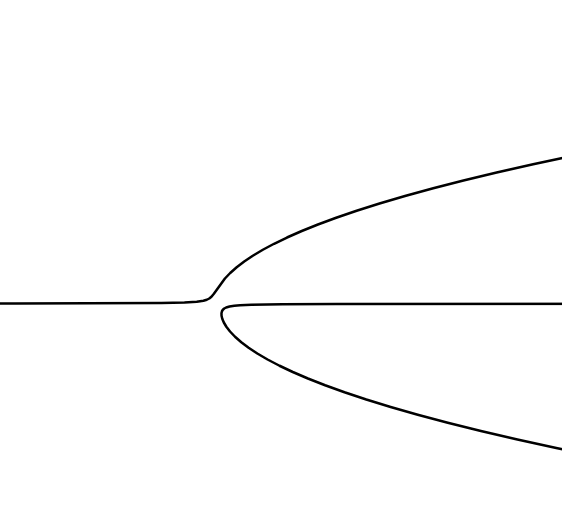
\includegraphics[width=0.3\textwidth]{figures/GEN_1.png}\hfill
    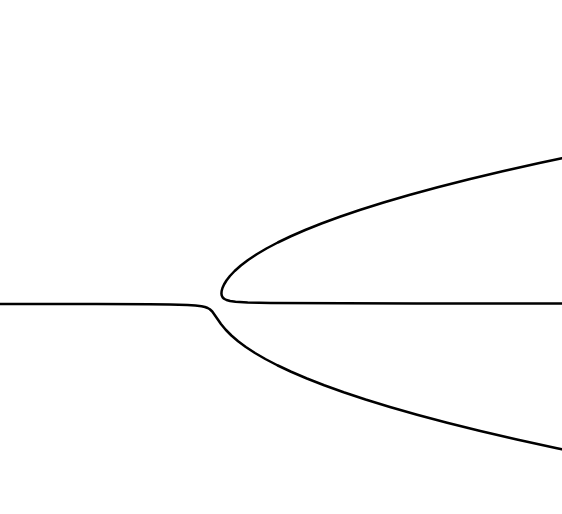
\includegraphics[width=0.3\textwidth]{figures/GEN_2.png}
    \caption{ $F^{-1}(-\varepsilon)$ et $F^{-1}(\varepsilon)$ pour la pitchfork }
    \label{fig:pitchfork_globale}
\end{figure}
Le corollaire précédent nous informe que les 
cas où un ensemble de niveau présente une 
bifurcation est "rare", et que la "plupart du 
temps"(de façon générique voir [SROUCE (mémoire de Thelma ?)]), il s'agit d'une variété. 

On aimerait 
bien avoir le pendant pour les paramètres, i.e 
que les bifurcations aient lieu en des valeurs 
singulières isolées, et que le lieu d'annulation 
soit "la plupart du temps" une variété de dimension $\operatorname*{Ind}(F)$. Ca n'est bien sûr pas vrai en général, même avec des fonctions non nulles: 

\begin{exemple}
    Considérez la fonction
    \begin{equation*}
        F: \R^2\rightarrow \R, (x,\lambda)\mapsto g(x)\lambda^2
    \end{equation*}
    avec $g(x)=e^{-\frac{1}{x}}\chi_{x>0}$. Il est clair que le lieu d'annulation est composé d'une droite horizontale connectée à un demi plan en $(0,0)$
\end{exemple}
\todo{Théorèmes de transersalités et généricité }


\subsection{Opérateurs de Fredholm différentiels}
Les opérateurs de Fredholm apparaissent très naturellement 

Nous rappelons qu'un multi-indice $\alpha$ de taille $n$ est simplement un tuple de nombres naturels $(\alpha_1,\cdots,\alpha_n)$ et qu'on a $D^{\alpha}=D^{\alpha_1}_1\cdots D^{\alpha_n}_n$, on pose aussi $|\alpha|=\sum_{i=1}^n \alpha_i$ et $\alpha !=\alpha_1!\cdots\alpha_n!$
\begin{definition}
    Soient $U$ un ouvert connexe de $\R^n$ et $m\geq 1$. Si pour tout $x\in U$, 
    $P(x,D)=\sum_{|\alpha|\leq m} c_{\alpha}(x) D^{\alpha}$ est un polynôme de degré $m$ en $D_1,\cdots,D_n$, $l\geq m\geq 1$ et $c_\alpha\in C^{l-m}(W,\R)$ avec $W$ un ouvert contenant $\bar{U}$ alors un opérateur de la forme 
    \begin{equation}\label{ellipticop}
        E: C^{l}(U;\R^p)\rightarrow C^{l-m}(U;\R^p), f 
        \mapsto \sum_{|\alpha|\leq m} c_{\alpha} D^{\alpha}f
    \end{equation}
    est appelé \coldef{opérateur différentiel 
    partiel} sur $U$.
    Et l'opérateur
    \begin{equation}\label{principalpart}
        f\mapsto \sum_{|\alpha|= m} c_{\alpha}D^{\alpha}f
    \end{equation}
    est la partie principale de  $E$ et les coefficients $c_
    {\alpha}$ avec $|\alpha|=m$ sont appelés coefficients 
    principaux
\end{definition}

Dans la suite, on dénotera par $P(x,D)$ un opérateur différentiel comme celui-ci dessus, et par $P_m(x,D)$ sa partie principale.
\begin{definition}
    L'opérateur $P(x,D)$  est \coldef
    {elliptique } en $x_0$ si $m=2p$ et si le polynôme $P(x_0,\xi)_m$ est 
    de signe constant sur $\R^n\setminus\left\{0\right\}$. Il est elliptique sur $U$ si il l'est en tout point de $U$ et 
    s'il existe un constante $c>0$ telle que 
    pour tout $x\in U$, on aie $P_m(x,\xi)\geq 
    c |\xi|^m$ alors il est  \coldef{uniformément 
    elliptique }
\end{definition}

En général, on étudie des problèmes du type
\begin{equation*}
    Ex=f\text{ sur $U$ et } \forall \alpha:|\alpha|\leq p-1, D^{\alpha}x|_{\partial U}=0 
\end{equation*}
En supposant typiquement que $U$ est une partie bornée de $\R^n$ ayant une frontière lisse et $E$ comme dans la définition précédente
\todo{Déplacer la définition des espaces de Hölder}



\newpage

\end{document}